\chapter{Background}
\label{chap:background}
This chapter covers technologies relevant to the thesis. It starts with an overview of similar monitoring tools for cluster-based applications and follows by a short overview of tools used for debugging of large-scale applications. Different approaches to applications profiling are described in the following part. 

In the next several sections the technologies considered to be used or used in the Distrace tool are introduced. The sections cover libraries for bytecode manipulation, communication, logging and also cover important relevant parts of Java libraries such as JNI and JVMTI. Docker is briefly described at the end of this chapter as it is used as the main distribution package of the whole platform.

\section{Cluster Monitoring Tools}
The most significant and relevant platforms on which this thesis is inspired are Google Dapper, Zipkin and HTrace. All three tools serve the same core purpose, which is to monitor large-scale Java-based distributed applications. Zipkin and HTrace are developed according to Google Dapper design and therefore these three platforms share a few similar concepts. The basic concept shared between the platforms is a concept called \textit{Span}. Spans are structures used to collect the shared state between the application nodes and usually encapsulate a few calls between the neighboring nodes with well-defined start and end of the communication. They are formed in hierarchical structures called trace trees, in which the user can see how distributed calls relate to each other. Spans are explained in more details later in the following sections. 

The following three sections describe the basics of each of the mentioned platforms. Since Zipkin, HTrace and Google Dapper share some basic concepts, only those parts of each platform that are relevant and interesting to the thesis are described.
\subsection{Google Dapper}
\label{dapper}
Google Dapper \cite{DapperPaper} is a proprietary software used by Google. It is mainly used as a tool for monitoring large distributed systems and helps with debugging and reasoning about applications performance running on multiple hosts at the same time. Different parts of the monitored system do not have to be written in the same programming language. Google Dapper has three main pillars on which is built:
\begin{itemize}
	\item \textbf{Low overhead} \newline
	Google Dapper should share the same life-cycle as the monitored application itself to capture also the intermittent events and thus low overhead is one of the main design goals of the tool.
	\item \textbf{Application level transparency} \newline
	The developers and users of the application should not need to know about the monitoring tool and are not supposed to change the way how they interact with the system when the monitoring tool is running. It can be assumed from the paper that achieving application level transparency at Google was easier than it could be in more diverse environments since all the code produced by Google use the same libraries and share similar control flow practices.
	\item \textbf{Scalability} \newline
	Such a system should perform well on data of significantly large scale.
\end{itemize}	
Google Dapper collects the information from distributed applications as distributed traces. The origin of the distributed trace is the communication or task initiator and the trace spans across the nodes in the cluster also participating in the computation or communication.
	
There were two proposed approaches for obtaining the distributed traces when Google Dapper was developed: black-box and annotation-based monitoring approaches. The black-box approach assumes no additional knowledge about the application whereas the annotation-based approach can make use of additional information via annotations. Google Dapper is mainly using black-box monitoring scheme since most of the control flow and RPC (Remote Procedure Call) subsystems are shared among Google, however, support for custom annotations is provided via additional libraries built on top of the core system. This gives the developer of an application possibility to attach some application-specific additional information to spans.
	
In Google Dapper, distributed traces are represented as so-called trace trees, where tree nodes are basic units of work referred to as spans. Spans are related to other spans via dependency edges. These edges represent the relationship between parent span and children of this span. Usually, the edges represent a set of related RPC calls or similar kind of communication. Each span can be uniquely identified using its id. In order to reconstruct the whole trace tree, the monitoring tool needs to be able to identify the span where the computation started. Spans without parent id are called root spans and serve exactly this purpose. Spans can also contain information from multiple hosts, usually from direct neighbors of the span. The structure of a span in Google Dapper platform is described in Figure \ref{fig:dapper_span}. The figure shows a single span encapsulating the client-server communication. It can be seen that events from both nodes are recorded within the single span.
\begin{figure}
	\centering
		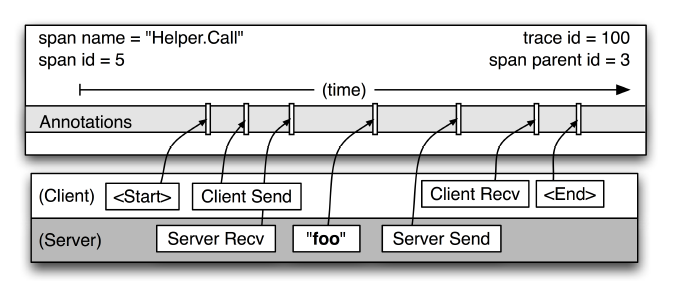
\includegraphics[scale=0.7]{dapper_span.png}
	\caption{Example of the span in Google Dapper, taken from Google Dapper paper \cite{DapperPaper}.}
	\label{fig:dapper_span}
\end{figure}

Google Dapper is able to follow distributed control paths thanks to instrumentation of a few common shared libraries used among Google developers. This instrumentation is not visible to the final users of the system and therefore Dapper has high-level of application transparency. Instrumentation in Dapper is achieved by tracing three main instrumentation points. 
\begin{itemize}
	\item Dapper attaches a so-called trace context as a thread-local variable to the current thread when the thread handles any kind of traced control path. Trace context is a small data structure containing mainly reference to a current and parent span via their ids.
	
	\item In distributed systems, the communication is often done via callbacks. A callback is a method which is usually executed when some execution in a different part of the application has finished. Dapper instruments the callback mechanism so when computation is deferred, traced callbacks still carry around the trace context of the creator and therefore also parent and current span ids.
	
	\item Most of the communication in Google is using single RPC framework with language bindings for different languages. This library is instrumented as well to achieve the desired application-level transparency.
\end{itemize}

The sampling of the captured data has also a positive effect on the low-level overhead of the whole application. As mentioned in the paper, the volume of data processed by Google is significant so only samples are taken.

\subsection{Zipkin}
\label{zipkin}
Zipkin\footnote{More information about Zipkin tracing tool is available at \url{http://zipkin.io}.} is an open-source distributed tracing system. It is based on Google Dapper technical paper and manages both the collection and lookup of the captured data. Zipkin uses instrumentation and annotations for capturing the data. Some
information is recorded automatically, for example, time when a span was created, whereas some are optional. Zipkin has also support for custom application-specific annotations.

Zipkin architecture can bee seen in Figure \ref{fig:zipkin_architecture}.
\begin{figure}
	\centering
	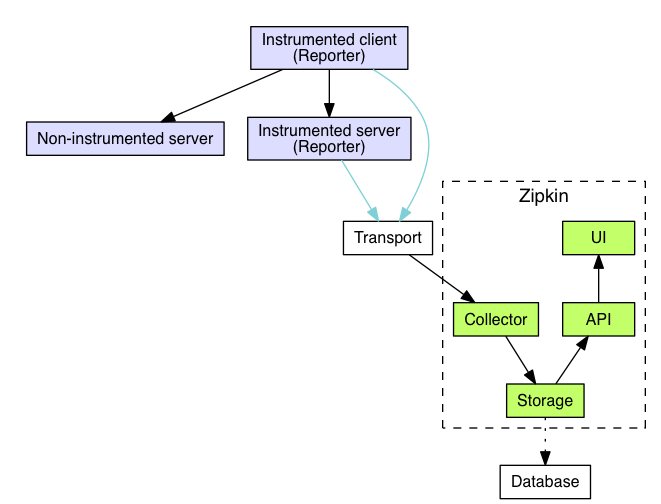
\includegraphics[scale=0.6]{zipkin_architecture.png}
	\caption{Zipkin architecture, from Zipkin Architecture \cite{ZipkinImage}}
	\label{fig:zipkin_architecture}
\end{figure}
The instrumented application is responsible for creating valid traces. For that reason, Zipkin has set of pre-instrumented libraries ready to be used in order to work well with the whole Zipkin infrastructure. Spans are stored asynchronously in Zipkin to ensure lower overhead. Once a span is created by the application, it is sent to Zipkin collector. In General, Zipkin consists of four components:
\begin{itemize}
	\item \textbf{Zipkin Collector} \newline
	The collector is usually a daemon thread or process which stores, validates and indexes the data for future lookups.
	\item\textbf{Storage} \newline
	Data in Zipkin can be stored in multiple ways which makes this a pluggable component. For example, data can be stored in Apache Cassandra\footnote{Apache Cassandra is a free and open-source distributed NoSQL database. It is designed to handle large amount of data and also provides high-availability.}, MySQL\footnote{MySQL is an open-source relational database system.} or can be send to Zipkin user interface right away without any intermediate storage. The last option is good for handling a small amount of data since the user interface is not supposed to handle storing data of big size.
	\item \textbf{Zipkin Query Service} \newline
	This component acts as a query daemon allowing the user to query various information about spans using simple JSON (Javascript Object Notation)\footnote{JSON is a lightweight data-interchangeable format based on object notation used in the Javascript programming language.} API.
	\item \textbf{Web User Interface} \newline
	A basic, but very useful user interface, which allows the user to see whole trace trees and all spans with dependencies between them. The user interface accepts the spans in JSON format. By default, it is available on port 9411.
\end{itemize}
The Zipkin web user interface is used as a front-end for the monitoring tool developed in the scope of this thesis. More information on how the user interface is used in the Distrace tool is described in more details in Section \ref{sec:zipkin_ui}.
 \subsection{HTrace}
 \label{htrace}
 HTrace\footnote{The project is available at \url{https://github.com/cloudera/htrace}.} is a tracing framework created by Cloudera used for monitoring distributed systems written in Java. It is based on Google Dapper as well and shares with Google Dapper the same concepts such as spans and trace trees. In order to allow tracing of the application, the users need to manually attach span identifiers to desired RPC calls (Remote Procedure Calls). These identifiers are then used to create relationships between spans collected on different nodes. HTrace stores the span and trace information in a thread-local storage and the user is responsible for making sure this state is transferred to a new thread or node. HTrace has also support for custom span annotations and thus allows the user to collect application specific information as part of the spans. 
 
 The disadvantage of this tool is the need for changing the code of the monitored application in order to allow the tracing and spans collection.
\section{Tools for Large-Scale Debugging}
Standard techniques and tools can be used for debugging distributed applications, however, the main purpose of these tools is to debug single node applications. Therefore, when applying them on nodes in the distributed application the information about dependencies between different nodes in the cluster is not available. Many tools for large-scale debugging exist, but this section just points out basic ideas behind two different approaches - discovering scaling bugs and behavior based debugging. 

\subsection{Discovering Scaling Bugs}
The scalability is one of the most important aspects of distributed systems. It is desirable to know how the platform scales when it process significantly large data and what is the expected scalability trend. It can happen that the platform can run significantly slower on big data than expected after testing on smaller data. This issue is usually called a scaling bug. Tools which can be used to help to discover scaling bugs are for example Vrishna and WuKong \cite{HPC}. Both of the mentioned tools are based on the same idea. They build a scaling trend based on data batches of a smaller size and the observed scaling trend acts as a boundary. The scaling bug becomes observable when the scaling trend is violated. The first tool, Vrisha, is not able to distinguish which part of the program violated the scaling trend. This is, however, possible in the second tool, WuKong. In comparison to Vrisha, WuKong does not build one scaling trend of the whole application but creates smaller models, each per some control flow structure in desired programming language. All these smaller models represent together the whole scaling trend. When the application observes the scaling bug, WuKong is able to locate the developer in the place in the code where the trend is probably violated.

\subsection{Behavior-based Analysis}
The second category of tools used for debugging large scale applications is based on behavior analysis. The basic idea behind these tools is creation of classes of equivalence from different runs and processes of the application. Using this approach, the amount of data used for further inspection is reduced down. These tools are especially helpful when discovering anomalies between different observed application runs. For example, STAT - Stack Trace Analysis Tool \cite{HPC}, is a lightweight and scalable debugging tool used for identifying errors on massive high-performance computing platforms. It gathers stack-traces from all parallel executions, merges together stack-traces from different processes that have the same calling sequence and based on that creates equivalence classes which make it easier for debugging highly parallel applications. 

The other tool used as the example in this category is AutomaDed \cite{HPC}. This tool creates several models from an application run and can compare them using clustering algorithm with (dis)-similarity metric to discover anomalous behavior. It can also point to a specific code region which may be causing the anomaly.

\section{Profiling Tools}
Profiling is a form of dynamic code analysis. It may be used, for example, for determining how long execution of each part of the system takes compared to the time of whole application run or for example to determine which part of the application uses the most memory. Profiling tools can be divided into two categories:
\begin{itemize}
	\item \textbf{Sampling Profilers} \newline
Sampling profilers take statistical samples of an application at well-defined points such as method invocations. The points where the application should take samples have to be inserted at the compilation time by the compiler. These profiles are good to collect information about time of how long a method run, caller of the method or for example the complete stack-trace. However, they are not able to collect any application specific information.
	\item \textbf{Instrumentation Profilers} \newline
The instrumentation profilers are based on the instrumentation of the application's source code. They record the same kind of information as the sampling profilers and usually give the developer the ability to specify extra points in the code where the application-specific data are recorded. 
\end{itemize}
 Sampling profilers usually have less overhead compared to instrumentation profilers, but on the other hand, instrumentation profilers allow to monitor application-specific parts of the application.
 
Profilers can be also looked at from different point of view and categorized based on the level on which they operate and are able to record the information.
\begin{itemize}
	\item \textbf{System Profilers} \newline
	System profilers operate on operating system level. They can show system code paths but are not able to capture method calls, for example, in Java application.
	\item \textbf{Application Specific Profilers} \newline
	Generally, application specific profilers are able to collect method calls within the application. For example, JVM profilers can show Java stack-traces but are not able to show the further call sequence on the operating system level.

\end{itemize}
The ideal solution for monitoring purposes of Java applications would be to have information from both kind of profilers, however combining outputs of these profiler types is not straightforward. The profilers used for collecting traces from both the operating system and JVM level are usually called mixed-mode profilers. JDK8u60 comes with the solution in a form of extra JVM argument \textit{-XX:+PreserveFramePointer} \cite{MixedModeProfilers}. The operating system is usually using this field to point to the most recent call on the stack frame and system profilers make use of this field. In case of Java, compilers and virtual machines don't need to use this field since they are able to calculate the offset of the latest stack frame from the stack pointer. That leaves this register available for various kind of JVM optimizations. The \textit{-XX:+PreserveFramePointer} option ensures that JVM abides the frame pointer register and does not use it as a general purpose register. Therefore, both system and JVM stack frames can appear in a single call hierarchy. Using the JVM mixed-mode profilers, it is possible to collect stack-traces leading to:
\begin{itemize}
	\item \textbf{Page Faults} - page faults are useful to show which JVM code triggered growth of the memory of the application.
	\item \textbf{Context Switches} - context switches are used to determine code paths that often lead to CPU switches.
	\item\textbf{Disk I/O Requests} - capturing Input/Output information allows us to see code paths leading, for example, to blocking seek operation on the hard-drive.
	\item \textbf{TCP Events} - these traces show code paths going from high-level Java code to low-level system methods such as \texttt{connect} or \texttt{accept}. They can be used to reason about the performance and good design of network communication in much better detail.
	\item \textbf{CPU Cache Misses} - information about cache misses can be used to optimize Java code to make better use of the existing cache hierarchy.
\end{itemize}

All the information above can be visualized using special graphs called Flame graphs.
\subsubsection{Flame Graphs}
Flame Graphs are special graphs introduced by developer Brendan Gregg. Flame graphs are visualization for sampled stack-traces, which allows the hot paths in the code to be identified quickly. The output of a sampling or instrumentation profiler can be significantly big and therefore, visualizing can help to reason about the performance in more comfortable way. The example flame graph is shown in Figure \ref{fig:flame_chart}.

\begin{figure}
	\centering
	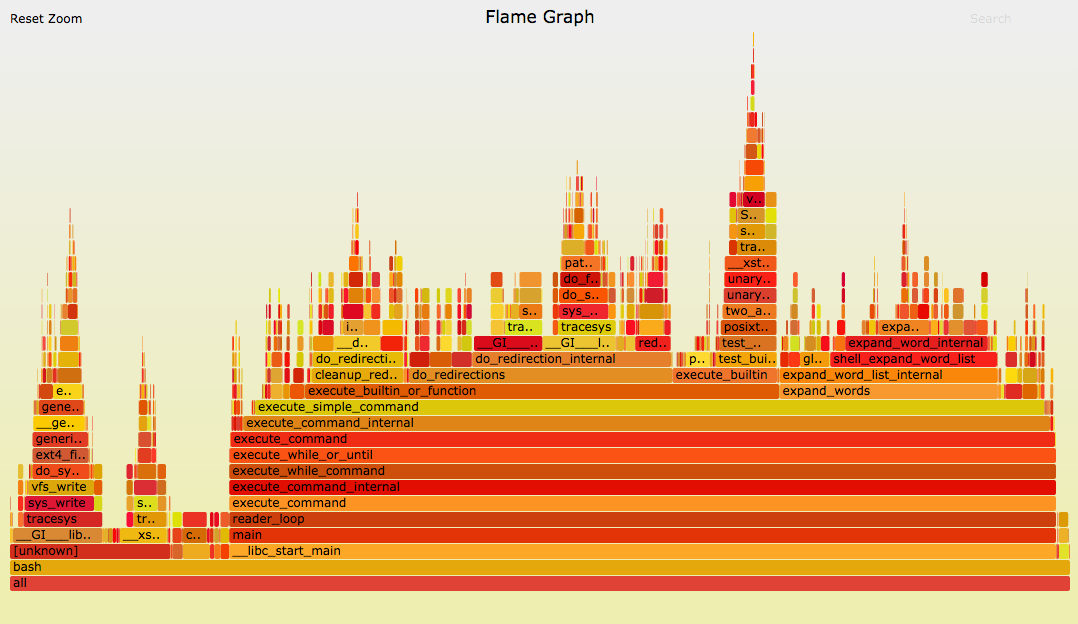
\includegraphics[scale=0.35]{flame_chart.png}
	\caption{Flame Graph example.}
	\label{fig:flame_chart}
\end{figure}
The flame graph is a graph where:
\begin{itemize}
	\item Each box represents a function call on the stack.
	\item The \textbf{y-axis} shows stack frame depth. The top function is the function which was at the moment of capturing this flame graph on the CPU. All functions underneath of it are its ancestors.
	\item The \textbf{x-axis} shows the population of traces. It does not represent the passage of time. The function calls are usually sorted alphabetically.
	\item The width of each box represents the time of how long the function spent on CPU.
	\item The colors are not significant, they are just used to visually separate different function calls.
\end{itemize}

Flame graphs can be created in a few simple steps, but it depends on the type of the profiler the user wants to use. The three steps are:
\begin{enumerate}
	\item Capture the stack-traces. For this step, the profiler of custom choice may be used.
	\item Fold stacks. The stacks need to be prepared so Flame graphs can be created out of them. Scripts for most of the major profilers exist and may be used to prepare the folded stack-traces. The scripts are available on the official page for the Flame Graphs.
	\item Generate the Flame graph itself using the helper script from the folded stack-traces.
\end{enumerate}

The purpose of this really short section is just to introduce the idea of Flame graphs because it's one of the future plans to add support for flame graphs into the Distrace monitoring tool developed in the scope of this thesis. For more information about the Flame graphs please visit the Brendan Gregg's blog\footnote{The blog is available at \url{http://www.brendangregg.com/flamegraphs.html}.}.
\section{Byte Code Manipulation Libraries}
Distrace highly depends on the Java bytecode instrumentation and this section gives an overview of four bytecode manipulation libraries considered to be used: Javassist, Byte Buddy, CGLib, and ASM. Since it's a core feature of the whole platform and affects both the performance and the usability of the Distrace tool, the chosen library was thoroughly reviewed before selected. The Byte Buddy library was selected and is therefore described in more details. The reasons for its selection are given in the following Chapter \ref{analysis}.

\subsection{ASM}
\label{asm}
ASM\footnote{The library is hosted at \url{http://asm.ow2.org}.} is a low-level high-performance Java bytecode manipulation framework. It can be used to dynamically create new classes or to redefine already existing classes. It works on the bytecode level so the user of this library is expected to understand the JVM bytecode in detail. ASM also operates on event-driven model as it makes use of Visitor design pattern\footnote{The visitor pattern is a way to separate data and the operations, which can be performed on the data.} to walk through complex bytecode structures. ASM defines some default visitors such as \texttt{FieldVisitor}, \texttt{MethodVisitor} or \texttt{ClassVisitor}. The ASM project can be a great fit for project requiring a full control over the bytecode creation or inspection since it's low-level nature.
\subsection{Javassist}
\label{javassist}
Javassist\footnote{Javassist library is hosted at \url{http://jboss-javassist.github.io/javassist/}.} is a well-known bytecode manipulation library built on top of ASM. It allows the Java programs to define new classes at run-time and also to modify class files prior the JVM loads them. It works on higher level of abstraction compared to ASM so the user of this library is not required to work with the low-level bytecode. The advantage of Javassist is that the injected code does not depend on the Javassist library at all. The code to be injected to the existing bytecode is expressed as instances of Java \texttt{String} class. The disadvantage of this approach is that the code to be injected is not subject to code inspection in most of the current IDEs. The strings representing the code are compiled at run-time by special Javassist compiler. This run-time compilation works well for most of the common programming structures but for example, auto-boxing and generics are not supported by the compiler \cite{JAVASSIST}. Also, it is important to mention that Javassist does not have support for the code injection itself. Therefore, it can be used for specifying the code which alters the original code but external tool needs to be used to inject the code itself.
\subsection{CGLib}
\label{cglib}
CGLib\footnote{CGLib library is hosted at \url{https://github.com/cglib/cglib}.} as another byte-code manipulation library built on top of ASM. The main concepts are built around \texttt{Enhancer} class, which is used to create proxies by dynamically extending classes at run-time. The proxified class is then used to intercept method calls and field access as is defined by the developer. However, CGLib lacks comprehensive documentation making it harder to even understand the basics.

\subsection{Byte Buddy}
\label{sec:byte_buddy}
Byte Buddy\footnote{Byte Buddy library is developed by Rafael Winterhalter and is freely available at \url{https://github.com/raphw/byte-buddy}. The page contains also a full API documentation and code examples.} is fairly new, light-weight and high-level bytecode manipulation library. The library depends only on visitor API of the ASM library which does not further have any other dependencies. It does not require from the user to understand format of Java bytecode, but despite this, it gives the users full flexibility to redefine the bytecode according to their specific needs. Despite it's high-level approach, it still offers great performance \cite{ByteBuddy_Perf} and is used at frameworks such as Mockito\footnote{Mockito is a mocking framework with a clean API allowing developers to write readable tests. More information is available at \url{http://mockito.org}.} or Hibernate\footnote{Hibernate is an open source Java persistence framework project and provides object-relational mapping in the Java programming language. More information is available at \url{http://hibernate.org}.}. Byte Buddy can be used for both code generation and transformation of existing code.

\subsubsection{Code Generation}
Code generation is done by specifying from which class a new class should be sub-classing. In the most generic case, class can be created based on the \texttt{Object} class. The newly created class can introduce new methods or intercept methods from its super class. In order to intercept existing methods (change their behavior and return value), the method to be intercepted has to be identified using instances of the \texttt{ElementMatchers} class. These matchers allow the developer to identify methods using, for example, their names, number of arguments, return types or associated annotations. The whole list of matchers and also examples how code can be generated is greatly described in the documentation of the Byte Buddy library.

The power behind Byte Buddy is also that it can be used to redefine classes at run-time. This is achieved by several concepts, mainly via Transformers, Interceptors and Advice API.
\subsubsection{Code Transformation}
\label{back:code_transform}
In order to tell Byte Buddy what method or field to intercept, the place in code which triggers the interception has to be identified. First, a class containing the desired method for instrumentation needs to be located. It can be done by simply specifying the class name or using more complex structures. For example, the element matchers may be used to only consider all classes \texttt{A} extending class \texttt{B} whilst implementing interface \texttt{C} at the same time. 

The next step is to define the \texttt{Transformer} class itself. Transformers are used to identify methods in the class, which should be instrumented, and they also specify the class responsible for the instrumentation itself. This class may be either Interceptor or Advice and their description is given in more detail in the following section. 

The methods to be instrumented can be specified in the transformer using the element matchers. In more detail, \texttt{AgentBuilder.Transformer} interface has a method \texttt{transform} which takes \texttt{DynamicType.Builder} as it's argument. This builder is used to create a single transformer wrapping all the transformers for all classes in the code so the result of this builder can be thought of as a dispatcher of the instrumentation for complete application.

There are two ways how to instrument a class in Byte Buddy. Either via Interceptors or via Advice API.
\subsubsection{Interceptors}
Interceptor is a class defining the new or changed desired behavior for the method to be instrumented.  The demonstration how Byte Buddy uses interceptors is shown on a small example. Let's assume the class \texttt{Foo} is the original unchanged class:
\begin{lstlisting}[language=Java]
class Foo {
	String bar() {
		return "bar"; 
	}
}
\end{lstlisting}
	
Let's also assume that the Interceptor is of type \texttt{Qux}. The interception of the class \texttt{Foo} using the defined interceptor looks like this in schematic code:

\begin{lstlisting}[language=Java]
class Foo {
	// Requires your interceptor class to be known
	static Qux $interceptor;
	String bar() {
		return $interceptor.intercept(); 
	}
	static {
		// Requires knowing the framework
		$interceptor = ByteBuddyFramework.defineField(Foo.class);
	}
}
\end{lstlisting}
		
It can, therefore, be seen that in the case of interceptors, Byte Buddy does not inline the bytecode to the \texttt{Foo} class but requires the interceptor class to be available on the machine where the instrumentation takes place. Also the interceptor field, in this case, \texttt{\$interceptor}, needs to be initialized before it is used for the first time. This is handled automatically by Byte Buddy framework using the special helper class called \texttt{LoadedTypeInitializer}. When the framework discovers that the instrumented class is about to be used for the first time, it initializes the static field to correct interceptor.

However, Byte Buddy also provides ways how to handle setting interceptors field manually. It is a more technical task but required for example in cases when the instrumentation is happening on a different machine where Byte Buddy framework is not available.
\begin{enumerate}
\item In Byte Buddy, the initialization strategy can be modified accordingly to the specific needs. The \textbf{no-op} strategy can be used, which has the effect of Byte Buddy not trying to initialize the interceptor fields. In this case, the user needs to handle the initialization. \texttt{LoadedTypeInitializer} instance can be recorded right before the class is about to be instrumented and this observed initializer can be used later for the initialization. This is especially useful in case the instrumentation happens in a different machine than in which the application is actually running. The initializer can be serialized together with the \texttt{Qux} \texttt{Interceptor} class to a machine with the application and a hook in the native agent can be created to call this initializer when the instrumented class is used for the first time.

\item Instead of referring to \texttt{Qux} as an instance, it can be delegated to as a static \texttt{Qux} class. In this case, no initializers have to be used since no interceptor field is required and the interception is performed via static methods. However, the interceptor class still needs to be known at run-time. This is demonstrated in a simple code bellow.

\begin{lstlisting}[language=Java]
class Foo {
String bar() {
// no need to have interceptor field
return Qux.intercept(); 
}
}
\end{lstlisting}

\item Instead of using Interceptors API, advice API which in-lines the code to the bytecode of the class itself may be used.
\end{enumerate}


\subsubsection{Advice API}
Advice API is another approach how code can be instrumented in Byte Buddy. This approach is more limited compared to the interceptors, but in cases where it's possible to use it, the code is in-lined into the bytecode of the original class and therefore no other dependencies are required. It is also stated in Byte Buddy documentation that performance of Advice API is better compared to the performance if interceptors.
However, the instrumentation using Advice API is only allowed before or after the matched method. This is achieved using the \texttt{Advice.onMethodEnter} and \texttt{Advice.onMethodExit} annotations. 

For example, the following method may be used as an advice: 
\begin{lstlisting}[language=Java]
class CustomAdvice {
   @Advice.OnMethodExit
   public static void exit(@Advice.This Callback callback) {
   	TraceContext tc = TraceContext.getFromObject(callback);
   	System.out.println("Method finished")
   	tc.closeCurrentSpan();
   }
}   
\end{lstlisting}

The method within a class on which the advice should operate needs to be defined. This is achieved by creating an instance of \texttt{Transformer} class which specifies the method to be instrumented.

\begin{lstlisting}[language=Java]
class CustomTransformer implements AgentBuilder.Transformer {

 @Override
 public DynamicType.Builder<?> transform(
			 DynamicType.Builder<?> builder,
			 TypeDescription typeDescription,
			 ClassLoader classLoader,
			 JavaModule module) {
   return builder.visit(Advice.to(CustomAdvice.class)
   .on(ElementMatchers.named("run")));
 }
}
\end{lstlisting}

Lastly, the class on which the transformer should operate needs to be defined. This is done on the main Byte Buddy instrumentation builder object in the following way:

\begin{lstlisting}[language=Java]
.type(is(Task.class))
.transform(new CustomTransformer())
\end{lstlisting}

Therefore, in this case, the \texttt{CustomAdvice} is applied on \texttt{Task} in the \texttt{run} method.
\section{Communication Middleware}
This thesis consists of several parts written in different languages that need to be able to communicate together. In order to arrange communication in such a heterogeneous environment, following libraries have been inspected.
\subsection{Raw Sockets}
\label{raw_sockets}
It this case raw sockets is not a library but it is referred to as using raw sockets on their low-level API. Using raw sockets has several advantages and disadvantages. It gives the user full flexibility and the highest possible performance since there isn't any additional layer between the application data and the socket itself. However, integrating different platforms and different languages can be time-consuming. Several frameworks have already been created to hide the implementation details of specific platforms so the user does not need to know about the language or underlying platforms differences.
\subsection{ZeroMQ}
\label{zeromq}
ZeroMQ\footnote{More information about the library is available at \url{http://zeromq.org}.} is a communication library built on top of raw sockets. The core of the library is written in C++, however binding into different languages exist. The library is able to transport messages inside a single process, between different processes on the same node or transfer messages over the network using TCP or also using multicast communication. The library also allows the user to create topologies using one of the many supported communication patterns. For example, publisher-subscriber or request-reply patterns are supported. The library has several benefits compared to raw sockets:
\begin{itemize}
	\item Hiding the differences between underlying operating systems.
	\item Message framing - delivering whole messages instead of a stream of bytes.
	\item Automatic message queuing. The internals takes care of ensuring the messages are sent and received in correct order. The user can send the messages without knowing whether there are other messages in the queue or not.
	\item Mappings to different languages.
	\item Ability to create different topologies. An example of a topology can be one-to-many communication pattern, where one socket can be connected to using multiple endpoints. 
	\item Automatic TCP reconnection.
	\item Support for zero-copy processing of messages.
\end{itemize}
\subsubsection{Zero-copy in ZeroMQ}
The library tries to apply a concept called zero-copy whenever possible. When high-performance is expected from a system or network, copying of data is usually considered harmful and should be minimized as possible. The technique of avoiding copies of data is known as zero-copy.

An example of data copying can be transferring data from a memory to a network interface or from a user application to an underlying kernel. It can be seen that zero-copy can't be implemented at all layers. For instance, without copying the data from the kernel to the network interface, no data could be actually exchanged. However, ZeroMQ can achieve zero-copy at least on the application message level so the users can create ZeroMQ messages from their data without any copying which is a significant performance benefit.
\subsection{Nanomsg}
\label{nanomsg}
Nanomsg\footnote{More information about the library is available at \url{http://nanomsg.org/}.} is a socket library shadowing the differences between the underlying operation systems. It offers several communication patterns, is implemented in C and does not have any other dependencies. Generally, it offers very similar features to ZeroMQ since it's heavily based on it.

Unlike ZeroMQ, Nanomsg matches the full POSIX\footnote{POSIX is a family of standards used to maintain compatibility between Unix-like operating systems by specifying a well-known interface for system methods \cite{POSIX}. } compliance. The author of the library states that since it's implemented in C, the number of memory allocations is drastically reduced compared to C++, where, for example, C++ STL containers are used  Also compared to ZeroMQ, objects are not tightly bound to particular threads. This gives the user flexibility to create their custom threading models without significant limitations. Nanomsg also implements zero-copy technique at additional layers which again leads to performance benefits compared to ZeroMQ \cite{Nanomsg_Diff}.

As in ZeroMQ, Nanomsq supports the following transport mechanisms:
\begin{itemize}
	\item \textbf{INPROC} \newline
	In-process communication is used for transporting messages within a single process, for example between different threads. In-process address is an arbitrary case-sensitive string starting with \texttt{inproc://}.
	\item \textbf{IPC}  \newline 
	Inter-process communication allows several processes to communicate on the same node. The implementation uses native IPC mechanism available on the target platform. 
	
	On Unix-like systems, IPC addresses are references to files, where both absolute and relative path can be used. The application has to have appropriate rights to read and write from the IPC file in order to allow the communication.
	
	 On Windows, the named pipes are used. The address can be an arbitrary case-sensitive string containing any character except the backslash. On both mentioned platforms, the address has to start with the \texttt{ipc://} prefix.
	\item \textbf{TCP} \newline
	TCP is used to transport messages in a reliable manner to a single recipient in a reachable network. The address in format \texttt{tcp://interface:port} has to be used when connecting to a node. When binding a node to a specific address, the address in format \texttt{tcp://*:port} has to be used.
\end{itemize}

Nanomsg can be used via the core C library, but several language mappings for different languages exist as well, which makes working with the library easier.
\subsubsection{C++11 Mapping}
Nanomsgxx\footnote{More information about Nanomsgxx mapping is available at \url{https://github.com/achille-roussel/nanomsgxx}.} a C++11 mapping for Nanomsg library. It is a small layer built on top of the core library making the API more C++11  friendly. Especially, there is no need to explicitly tell when to release resources, since it's handled automatically in the class descriptors. The \texttt{nnxx::message} abstraction over Nanomsg \texttt{nn::message} automatically manages buffers for zero-copy and also errors are reported using the exceptions which are sub-classes from \texttt{std::system\_error}.
\subsubsection{Java Mapping}
Several Java bindings of Nanomsg library exists, but only jnanomsg library\footnote{More information about jnanomsg mapping for Nanomsg library is available at \url{http://niwinz.github.io/jnanomsg/latest/}.}  is described here. This language binding is built on top of JNA (Java Native Access)\footnote{Java Native Library is a library allowing to use native shared libraries from Java without using JNI or native code. For more information about the library, please see \url{https://github.com/java-native-access/jna}.} library. It offers all the functionalities offered by the core library, but also introduces non-blocking sockets exposed via a callback interface.

\section{Java Libraries}
This section describes some fundamental Java-related libraries and technologies on which this thesis heavily depends. Firstly, Java Virtual Machine Tool Interface (JVMTI) is described, followed by the basic introduction to the Java Native Interface.
\subsection{JVMTI}
\label{JVMTI}
The JVM Tool Interface is an interface used by development and monitoring tools for communication with JVM. It allows the user to monitor and control the application running in Java virtual machine. An application communicating with the JVM using JVMTI is usually called an agent. Agents are notified via events occurring inside JVM and can react upon them. Agents run in the same process as the application itself, which reduces the delay in the communication between the application and the agent. Since JVMTI is an interface written in C, agents can be written in C or C++. 

JVMTI supports two modes of how an agent can be started. It can be started either in \textbf{OnLoad} phase or in \textbf{Live} phase. In the \textbf{OnLoad} phase, the client is started together with the application and agent location can be specified using 2 arguments:
\begin{itemize}
	\item \texttt{-agentlib:<agent-lib-name>=<options>} \newline
	In this case, the agent library name to load is specified and it is loaded using platform specific manner.
	\item \texttt{-agentpath:<path-to-agent>=<options>} \newline
	In this case, the path to a location of the agent library is specified and the agent is loaded from there.
\end{itemize}

In the \textbf{Live} phase, the agent is dynamically attached to a running application. This approach is more flexible since it is not required to attach the agent library to the monitored application in advance. However, it brings several limitations as well.

The goal of this section is not to describe full JVMTI functionality, but just give the reader a brief introduction to the interface. For more details about JVMTI, please visit the official documentation\footnote{The official JVM Tool Interface documentation describes the full API and is available at \url{https://docs.oracle.com/javase/7/docs/platform/jvmti/jvmti.html}.}. The following sections try to briefly describe the important parts of JVMTI relevant to the thesis.

\subsubsection{JVMTI Agent Initialization}
\label{subsec:jvmti_init}
When an agent is started, the following JVMTI method is always called: \linebreak \texttt{Agent\_OnLoad(JavaVM *jvm, char *options, void *reserved)}. This method should contain the agent initialization specific for the application. Usually, the agent initialization process consists of several phases:
\begin{enumerate}
	\item Optionally, parse arguments passed to the JVMTI agent.
	\item Initialize JVMTI environment in order to be able to communicate with the observed application. JVMTI does not handle threads switches automatically, so proper locking and thread management fully depend on the user code.
	\item Register capabilities of the JVMTI agent. The capabilities specify what are the operations the JVMTI agent can perform. The agent can be, for example, allowed to re-transform classes or react to different class hook events.
	\item Register events the agent should react to. JVMTI does not inform the agent about all events by default, these events have to be manually defined.
	\item Register callbacks for the events the agent is interested in. Even though the JVMTI supports more events, the interesting events are: 
		\begin{itemize}
			\item \texttt{cbClassLoad}
			\item \texttt{cbClassPrepare}
			\item \texttt{cbClassFileLoadHook}
			\item \texttt{callbackVMInit}
			\item \texttt{callbackVMDeath}
		\end{itemize}
	\item Optionally, initializing phase is also good for creating locks which may be later used for synchronization between different JVMTI threads.
\end{enumerate}

The user of JVMTI is also required to manually implement queuing and locking when processing multiple JVMTI events at the same time since the framework is not designed to handle these cases. \cite{JVMTI_Callbacks}.
\subsubsection{JVMTI basic callbacks}
As mentioned above, there are several events sent from the observed Java application. When instrumenting the code of the applications, the following callbacks are used to capture the mentioned events.
\begin{itemize}
	\item \texttt{cbClassLoad} - triggered when a class has been loaded by target JVM.
	\item \texttt{cbClassPrepare} - triggered when a class has been prepared by target JVM. All static fields, methods, and implemented interfaces are available at this point, but no code has been executed at this phase.
	\item \texttt{cbClassFileLoadHook} - triggered when the virtual machine obtains class file data, but before the class is loaded. Usually, class instrumentation is based on this hook, since the callback contains output argument for the instrumented bytecode.
	\item  \texttt{callbackVMInit} - triggered when virtual machine is initialized.
	\item  \texttt{callbackVMDeath} - triggered when the virtual machine has been closed. This event is triggered in both planned and forcible stop.
\end{itemize}

\subsection{JNI}
\label{JNI}
Java Native Interface is a framework allowing Java code running in Java Virtual Machine to call native applications ( usually written in C or C++ ). It also allows native applications to access and call Java methods. All JNI operations require an instance of class \texttt{JNIEnv} to be available. This environment is always bound to a specific thread and manages the connection to the Java virtual machine. When calling a Java method from the native application, the correct method has to be first found. This is achieved by specifying the types and method signature of the method.
\subsubsection{Java Types Mapping}
For each Java primitive type, there is a corresponding native type in JNI. Native types always start with the \textbf{j} as the prefix, for example, \texttt{boolean} is a Java type whereas \texttt{jboolean} as a native type.
All other JNI reference types are referred to via \texttt{jobject} class. This means that Java arrays are accessed as \texttt{jobject} as well since at this level they are referred to as Java objects. The most important question is how the types in method signatures can be specified. There is a mapping assigning each type a signature, which is used exactly for this purpose. The following Table \ref{mapping_jni} is based on the JNI documentation\footnote{The original and more complete documentation for JNI types mapping is available at \url{http://docs.oracle.com/javase/7/docs/technotes/guides/jni/spec/types.html}.}. and describes the mapping in detail:
\begin{center}
\begin{tabular}{ l l }
	  \hline
	  Type Signature & Java Type \\ \hline
	Z & boolean \\
	B & byte \\
	C & char \\
	S & short \\
	I & int \\
	J & long \\
	F & float \\
	L fully-qualified-class ; & fully-qualified-class \\
	{[} type & type{[]}\ \\
	( arg-types ) ret-type & method type \\
\end{tabular}
\captionof{table}{Mapping type signatures to Java types.}\label{mapping_jni}
\end{center}

For example, the method: \newline \texttt{xx.yy.Person foo(int n; boolean[] arr, String s);} has the following signature:
\texttt{(I[ZLjava/lang/String;])Lxx/yy/Person;}

Note that in JNI, the path elements in the fully qualified class name are separated by slashes instead of dots.
\subsubsection{Example JNI Method Call}
The method bellow demonstrates how JNI can be used to call a Java method \texttt{getClassLoader} from the native environment.

\begin{lstlisting}[language=c++]
        jobject getClassLoaderForClass(JNIEnv *jni, jclass clazz){
        // Get the class object's class descriptor
        // (jclass inherits from jobject)
        jclass clsClazz = jni->GetObjectClass(clazz);
        // Find the getClassLoader() method in the class object
        jmethodID methodId = jni->GetMethodID(
		        clsClazz,
		        "getClassLoader", // name of the Java method
		        "()Ljava/lang/ClassLoader;"); // method signature
        return (jobject) jni->CallObjectMethod(clazz, methodId);
        }
\end{lstlisting}

It can be seen that the reference to the method needs to be obtained at first. This reference is used later for the method invocation itself. For the performance reasons, it is a good practice to cache the references to Java methods or objects which are accessed from JNI often, since creating the reference has some initial overhead.

\subsection{Relevant Aspects of the  Java Language}
This section covers selected areas of the Java programming language and run-time platform relevant to the thesis. It briefly describes the class loading process for dynamically loaded classes. This is followed by the explanation of two important class loaders relevant to the thesis and lastly, \texttt{ServiceLoader} class is shortly described.
\subsubsection{Class Loading Process}
Java allows programs to load classes dynamically at run-time. This is achieved by the following process:
\begin{enumerate}
	\item \textbf{Loading} - Load the bytecode from a class file.
	\item \textbf{Linking} - Linking is the process of incorporating a new class to the run-time state of the JVM. This phase consists of three sub-phases:
	\begin{enumerate}
		\item \textbf{Verification} - Ensure that type in the binary format is correct and respects JVM restrictions.
		\item \textbf{Preparation} - This phase mainly allocates the memory for fields inside the loaded type.
		\item \textbf{Resolution} - This phase is optional and depends on JVM implementation. Resolution is the process of transformation symbolic references in the type's constant pool into direct references. The implementation may decide to behave in a lazy way and delay resolution for the time when the type is accessed for the first time or behave in an eager way and resolve all types in advance. Constant pool contains all references to variables and methods, found during the compilation time, in the class file.
	\end{enumerate}
	\item \textbf{Linking Phase} - class (static) variables are initialized to initial values.
\end{enumerate}
\subsubsection{Relevant Class Loaders}
There are several class loaders used natively in Java. However, this section describes only two, which are referenced later in the thesis. 

\begin{itemize}
	\item\textbf{Bootstrap class loader} \newline
	This class loader is used to load system classes. When using the native agent, even classes loaded by bootstrap class loader can be instrumented and thus behavior of standard Java classes can be changed.
	
	\item  \textbf{sun.reflect.DelegatingClassLoader} \newline
	This class loader is used on the Oracle JVM as the effect of a mechanism called \textit{inflation} \cite{inflation}. Usually, reflective access to a method or a field is initially performed via JNI calls. When Oracle JVM determines that there is a repetition in calling the same method or the same field via JNI ( reflection), it creates a synthetic class\footnote{Class created dynamically at run-time}, which is used to perform this call without the JNI. This has initial speed overhead, but at the end, it speeds up the reflection calls. The classes created for this purpose are loaded and managed by exactly this class loader. 
\end{itemize}
\subsubsection{ServiceLoader Class}
\texttt{ServiceLoader} class is used to locate and load service providers. The service provider is an implementation of a service that is usually defined as a set of methods inside an abstract class or interface. 

Service loader is used to load specific service providers at run-time. The group of service providers to be loaded can be specified via the service type, usually type of an interface or abstract class. The available service providers have to be defined in the META-INF folder of the application's JAR (Java Archive) distribution. For example, imagine there are service A and two implementations, \texttt{Impl1} and \texttt{Impl2}. In that case, META-INF folder should contain text file named A containing lines:
\begin{center}
\texttt{Impl1} \newline
\texttt{Impl1}  \newline
\end{center}
As a result, service loaders can be used to extend the application capabilities without changing the source code. When a new implementation of a service should be supported, it just needs to be registered inside the META-INF folder and the application will automatically use the new service provider together with the rest of the service providers defined earlier.
\section{Logging Libraries}
Logging can have a negative effect on the performance of the application, but sometimes it's necessary to have information from various application runs to be able to locate bugs or discover the wrong configuration. Since one of the thesis's requirements is low-overhead, the selection of logging library is important for the performance of the Distrace as well. 

Spdlog\footnote{More information about Spdlog is available at \url{https://github.com/gabime/spdlog}.} is a fast, header only logging library written in C++11 on which this project is based on. It allows both synchronous and asynchronous logging and custom message formatting.
\section{Docker}
Docker\footnote{More information about Docker is available at \url{https://www.docker.com}.} is an open source project used to pack, ship and run any application as a lightweight container. It is used to package applications in prepared environments so the user does not need to worry about configuration and downloading the correct dependencies for the application. 

Docker Compose is an extension built on top of Docker allowing the user to specify multi-container startup script. This script can define dependencies between different containers which leads to a simple and automated way how to start a group of related applications in separated environments using one single call. 

